\documentclass{article}
% ########### PAQUETES% ###########
\usepackage[utf8]{inputenc}
\usepackage[spanish]{babel}
\usepackage[linktoc=all]{hyperref}

\usepackage{graphicx}
\usepackage{caption}
\usepackage{float}

\usepackage[dvipsnames]{xcolor}

\usepackage{import} %reemplaza a input incluyendo el path relativo al archivo importado
\usepackage{soul}   %otros formatos de texto, \st tachado
%------------------- Dimensiones -------------------
\usepackage{geometry}
\geometry{a4paper, total={170mm, 240mm}, top=20mm, left=20mm}
\setlength{\headheight}{15mm}% ...at least 51.60004pt
\setlength{\footskip}{15mm}% ...at least 51.60004pt
%----------------------------------------------------

%------------------- Encabezado y Pie de pág -------------------
\usepackage{fancyhdr}
\pagestyle{fancy}
\fancyhf{}
\lhead{Cátedra de Proyecto Final}
\rhead{Carpeta de campo}
\rfoot{Página \thepage}
%---------------------------------------------------- % 
% #################################
\begin{document}
% ####### PORTADA #######
%---------------------- INICIO CARATULA ----------------------
\begin{titlepage}
 \centering
	
\includegraphics[scale=0.80]{imagenes/logo_utn.jpg} \par
 	\vspace{1cm}
 	{\scshape\LARGE Universidad Tecnológica Nacional \par}
 	{\scshape\large Facultad Regional de Córdoba \par}
 	\vspace{1cm}
 	{\Large Cátedra de Proyecto Final \par}
	\vspace{0.5cm}
	{\bfseries \LARGE Tesis de Grado \par}
	\vspace{0.5cm}
	 {\bfseries \Large ``Carpeta de campo." \par}

 	\vspace{1.5cm}

	\begin{tabular}{ll}
	    Castro, Franco          &   67432 \\
	    Cussa, Mayco            &   66871 \\
		Navarro, Facundo 	    &	63809 \\
		Nobile, Jonathan        &   69325 
	\end{tabular}
	
	\vspace{1cm}
	
 	\vfill

	Docentes: \\
        Ing. Encina, Lucas \\ 
        Ing. Galleguillo, Juan Cayetano del Corazón \\
        Ing. Gaydou, David 
        
 	\vfill
	{\large \today\par}
\end{titlepage}
%---------------------- FIN CARATULA ----------------------
% #######################

\section{Introducción a la problemática}
\begin{figure}[ht]
\centering
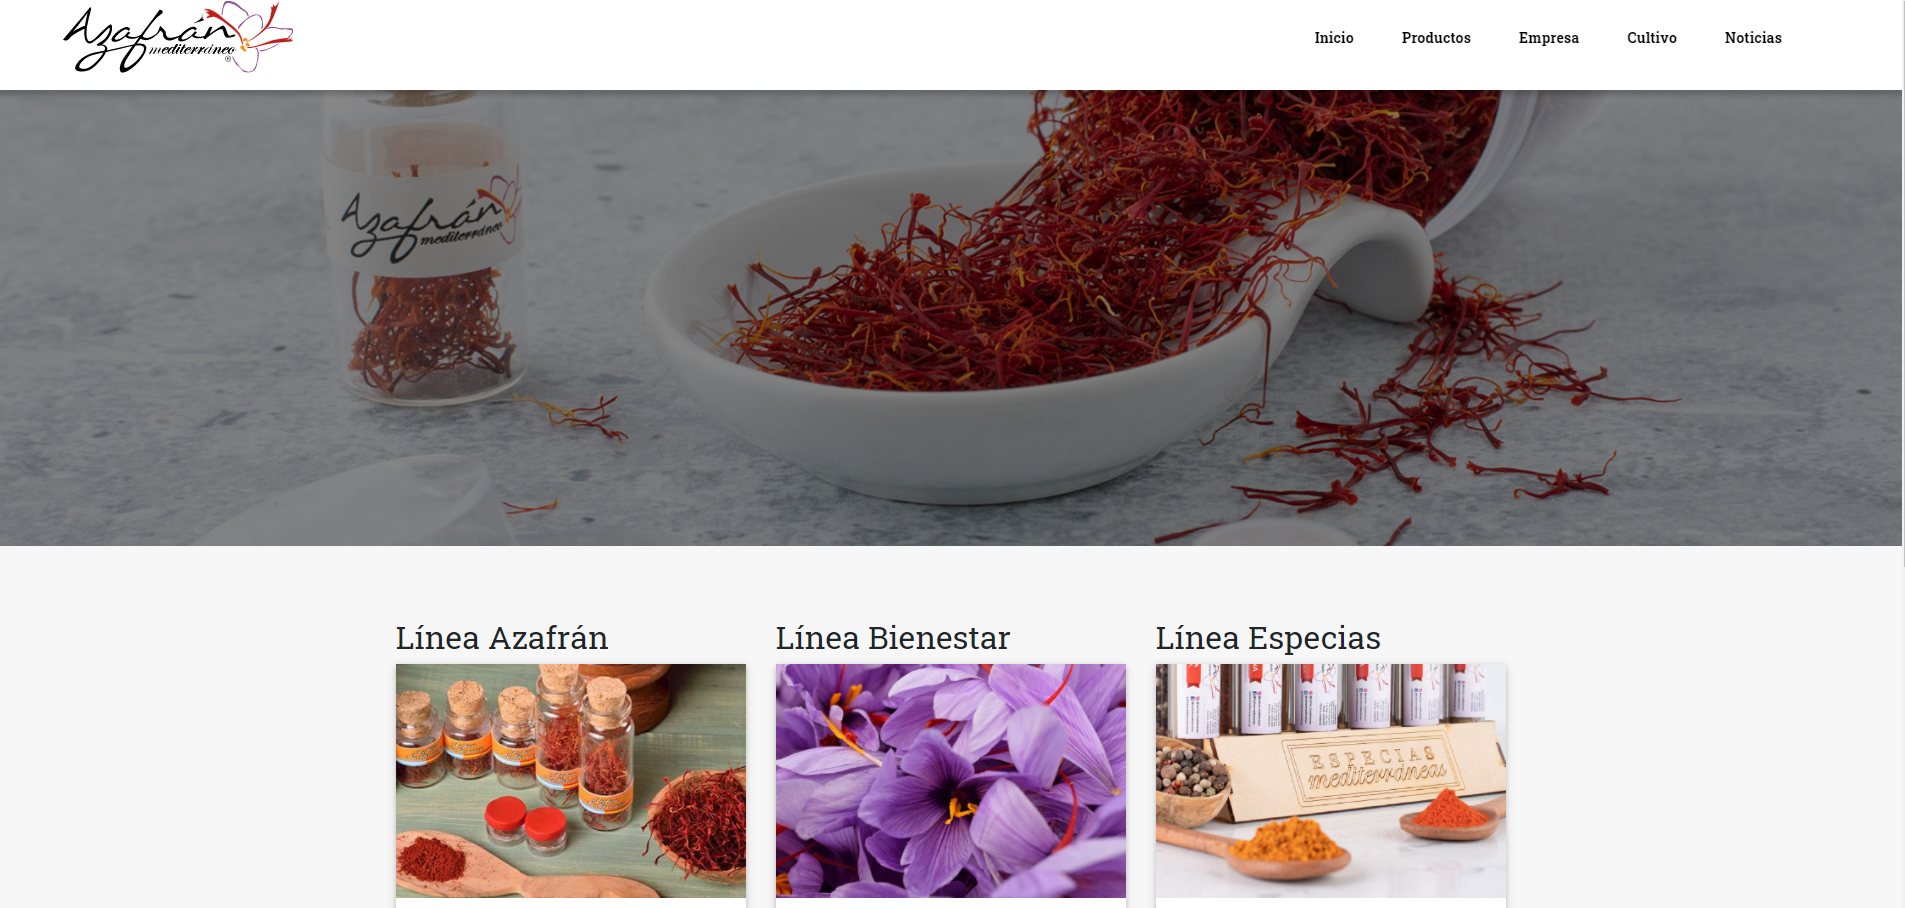
\includegraphics[width=\textwidth]{Imagenes/Azafran.png} \par
\end{figure}

La idea de nuestro proyecto surge en base a la necesidad de la empresa \textbf{Azafrán mediterráneo} de mejorar el rendimiento de sus cultivos.

En la zona de Valle de Calamuchita, a unos 10km de la localidad de `Los Reartes', se establecieron hace unos años cultivos de azafrán, primero en una pequeña escala, llegando a aumentar hasta 10 veces su volumen de producción en la actualidad. 

La empresa eligió desarrollar sus cultivos en esta zona debido a su clima frió y seco, ya que las raíces de las plantas de azafrán son muy susceptibles a la proliferación de un hongo, lo que deriva en una importante pérdida en volumen de producción, cercana al 30\% anual, y consecuentemente un gran impacto en las ganancias netas, con montos que llegan a alcanzar los millones de pesos. En base a investigaciones que llevaron a cabo los dueños de estos campos en conjunto con ingenieros agrónomos de la Universidad Nacional de Córdoba, se determinó que la aparición de estos hongos se produce para determinados valores de humedad y temperatura del suelo, por lo que se volvió una necesidad imperativa tener un monitoreo estricto y preciso de estas variables en todo momento.

\begin{itemize}
    \item \href{https://www.infoagro.com/aromaticas/azafran2.htm}{\textit{Información sobre el Azafrán}}
\end{itemize}


\section{Objetivo}
Llevar a cabo el desarrollo de una central que se encargue de realizar procesos de adquisición de estas variables de suelo mediante sensores, para su posterior carga en un servidor, y que de esta manera el productor pueda controlar estos parámetros en tiempo real. Además este sistema debe ser capaz de activar una serie de circuitos de riego por goteo, con el fin de mantener la humedad y temperatura de suelo en el rango requerido.

\section{Propuesta técnica}

Al encender la central con un botón, se indicara con una señal lumínica. Luego se prende la pantalla y se muestran los parámetros medidos por los sensores, en base a los mismos se accionaran o no las electroválvulas para mantener los niveles de humedad y temperatura, dando aviso a través una señal sonora. A su vez también se enviaran los valores a un servidor para que el usuario pueda acceder desde cualquier dispositivo conectado a internet.
Con el teclado se podrá navegar sobre el menú de la pantalla para establecer cronogramas de riego.


\section{Requisitos específicos}
Como mencionamos anteriormente, las raíces de las plantas de azafrán son muy sensibles a la proliferación de un hongo que crece ante determinadas condiciones de humedad y temperatura. Estas fueron determinadas luego de extensas investigaciones realizadas por ingenieros agrónomos y biólogos de la Universidad Nacional de Córdoba, quienes pautaron los parámetros a evitar en pos de la salud de los cultivos.
Esta investigación definió que los hongos nacen para las siguientes condiciones:


\begin{itemize}
    \item Temperatura mayor a $23^\circ$C por un tiempo mayor a 3 días.
    \item Humedad mayor a 75\% por un tiempo mayor a 2 días.
\end{itemize}

Partiendo de estos datos se diseñará nuestro sistema para tratar de mantener las variables de suelo en rangos prudentemente alejados de estos valores, empleando el riego para bajar la temperatura del suelo en lugar de su uso para la irrigación tradicional.

Otro dato importante a tener en cuenta es que los cultivos de azafrán no se realizan en el suelo como sucede con las demás plantas, sino que se emplean cajones o canteros elevados a un metro del suelo, ya que tanto la siembra como la cosecha se realizan a mano, haciendo esto un proceso mas ameno. Como consecuencia de este proceso manual la distribución de los bulbos es completamente uniforme y conocida, distribuyéndose equidistantes entre sí y a una profundidad de \textbf{5 centímetros}. En sí, estos son datos muy importantes para nosotros porque nos proporcionan un entorno mucho mas controlado en cuanto a lo que respecta composición y compactación del suelo, teniendo también características de irrigación mejor definidas a lo que serían si se realizara de forma tradicional.

\begin{figure}[h!]
    \centering
    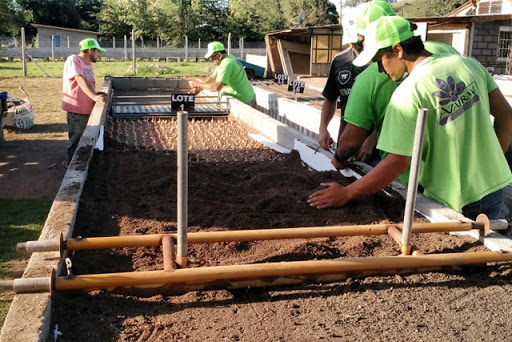
\includegraphics[width=\textwidth]{Imagenes/cantero.png}
    \caption{Canteros empleados para cultivo de azafrán.}
    \label{fig:my_label}
\end{figure}


\section{Investigación empírica}

Para el desarrollo de este proyecto, se identificó como uno de los puntos claves y críticos a los sensores que se encargaran de hacer la adquisición de humedad de suelo. Ante esto procedimos a hacer una extensa investigación, acompañada de numerosas pruebas cuyo objetivo fue comprobar la veracidad de los datos recopilados.


\subsection{Sensores Resistivos}

En base a lo anterior se optó en una primera instancia, por el uso de sensores de carácter resistivo, debido a su bajo costo y a la gran cantidad de foros y páginas web que los recomiendan. Adquirimos varios modelos para ponerlos a prueba, siendo algunos de ellos los que se ven en la Figura \ref{fig:sensores_resistivos}. 

\begin{figure}[H]
    \centering
    \subfloat[FC-28]    {{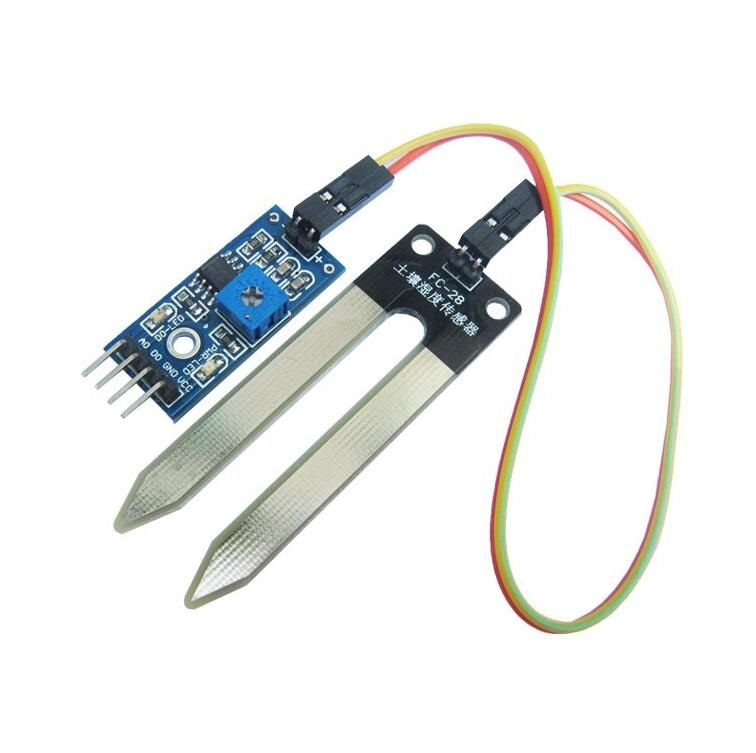
\includegraphics[width=5cm]{Imagenes/resist1.jpg} }} \label{fig:res_1}
    \subfloat[HR202]  {{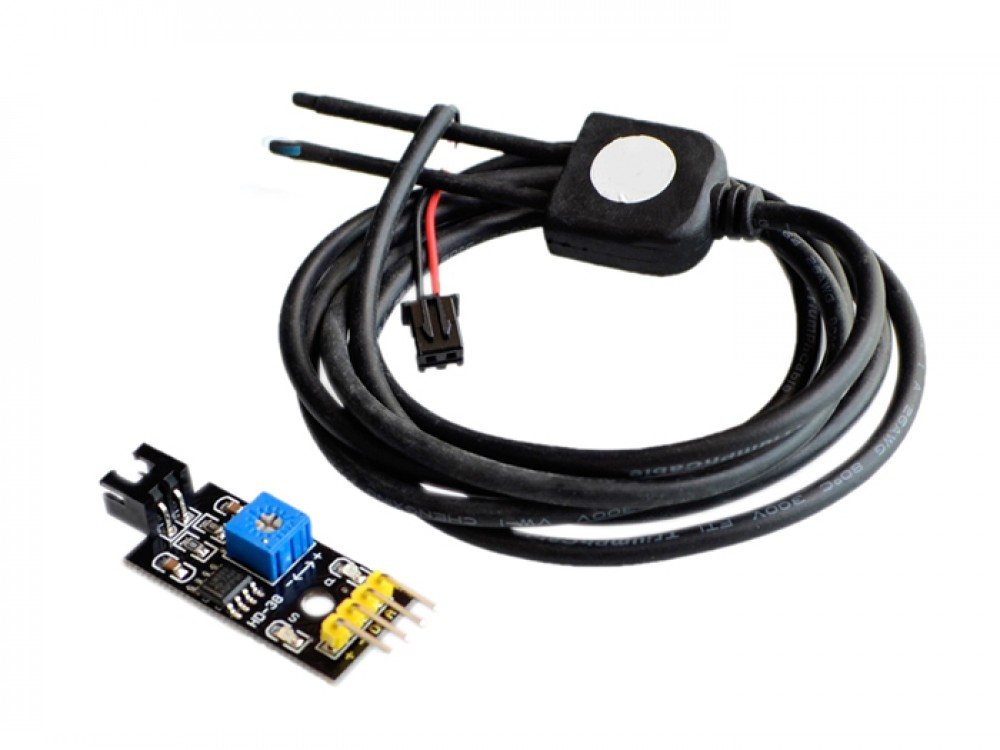
\includegraphics[width=5cm]{Imagenes/resist2.jpg} }} \label{fig:res_2}
    \caption{Sensores resistivos implementados.}%
    \label{fig:sensores_resistivos}%
\end{figure}

Al momento de usarlos nos dimos con un gran numero de inconvenientes. El primero de ellos tenía que ver con la veracidad y repetibilidad de las mediciones, ya que su principio de funcionamiento se basa en hacer circular una corriente entre las dos terminales del sensor, incrementando este valor proporcionalmente a la humedad y viceversa. El problema aquí era que este método es muy sensible al cambio de variables del sistema que afecten a la conductividad del suelo, debido a que si se empleaba un agua con mayor o menor concentración de minerales, si cambiaba el suelo o el tipo de fertilizante, también lo hacia el valor medido por este componente, haciéndolo inviable para cualquier tipo de aplicación seria. Además de lo anterior, el hecho de estar circulando corriente a través de las patas del dispositivo, sumado a que se encuentra expuesto en un entorno agreste, terminaba produciéndose un fenómeno de electrólisis que conllevaba a la degradación y oxidación de nuestros sensores.

\subsection{Sensores Capacitivos}
Luego de la experiencia anterior, decidimos cambiar la tecnología de medición, pasando a utilizar sensores de tipo capacitivo como se puede observar en la Figura \ref{fig:sensor_capacitivo}. El principio de funcionamiento de este dispositivo es muy similar al de los resistivos mencionados, donde sobre un PCB se plasma una pista con forma de 'U', la cual cuenta con una capacitancia que se encuentra determinada por el material que la rodea, en este caso tierra. A medida que el suelo se moja, este valor de capacitancia se altera debido al cambio en el dieléctrico, lo cual se transforma en valores de tensión que se interpretan para realizar una escala de valores de humedad. 
Al momento de probar estos sensores, encontramos que se repetía el mismo inconveniente que en los resistivos, en el cual el PCB terminaba deteriorándose rápidamente, además de arrojar mediciones inestables e inconsistentes, que a pesar de ser mejores que en los resistivos se concluyó que tampoco eran apropiados para nuestro proyecto.

\begin{figure}[H]
    \centering
    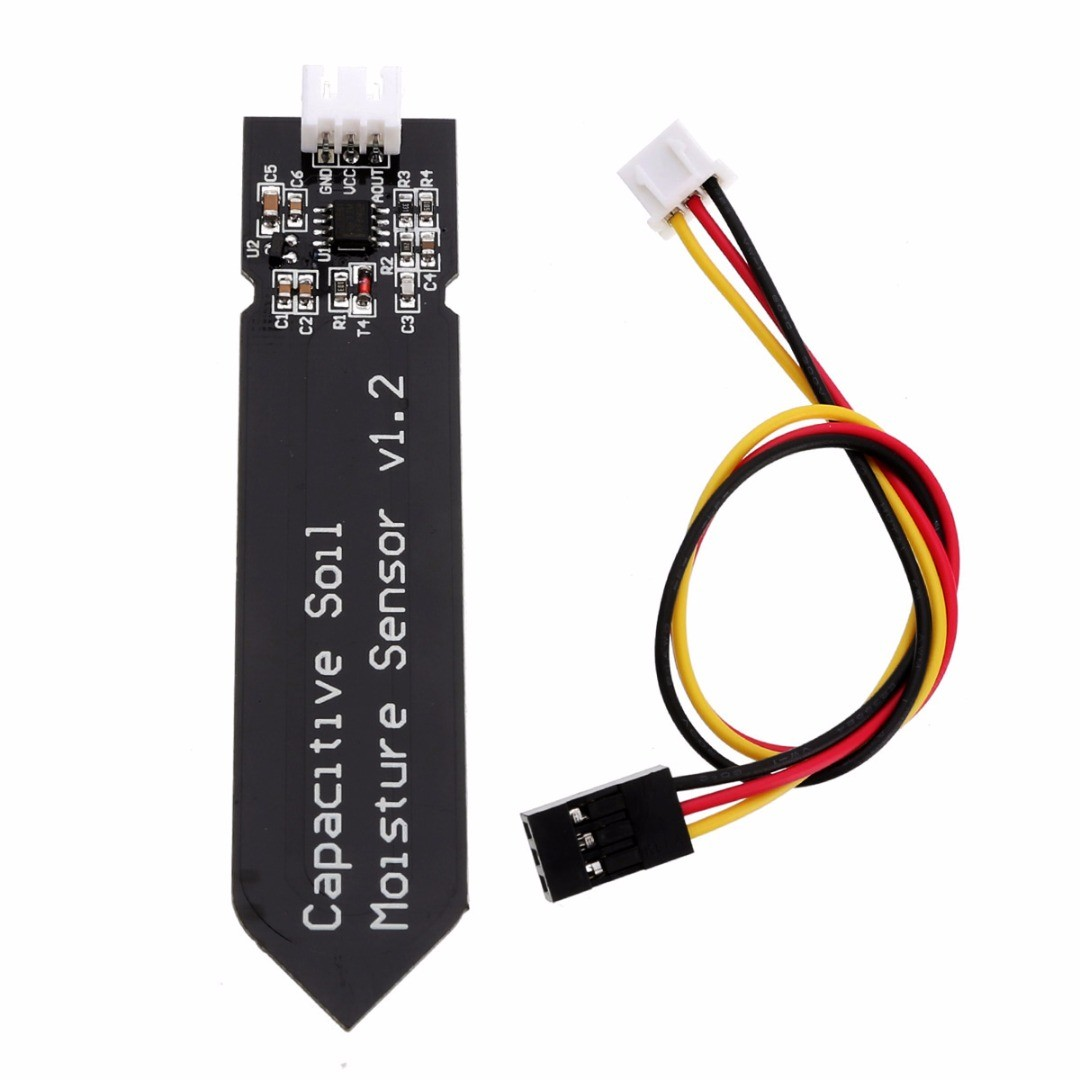
\includegraphics[scale=0.15]{Imagenes/capa1.jpg}
    \caption{Capacitive Soil Moisture Sensor V1.2}
    \label{fig:sensor_capacitivo}
\end{figure}

\subsubsection{Sparkfun SHT11}
Basándonos en toda la investigación y evidencia recopilada a lo largo de estas experiencias, decidimos realizar pruebas con otro tipo de sensor capacitivo debido a que esta tecnología mostró un mejor comportamiento que su contra-parte resistiva. Para este caso optamos por un sensor de mayor costo y calidad, al rededor de diez veces el de los otros dispositivos.
Este sensor es el SHT11 de la compañía `Sensirion', y además de ser capacitivo y tener una resolución mucho superior a los que probamos anteriormente, incorpora en su encapsulado un sensor de temperatura, resolviendo otro gran problema de nuestro proyecto. Mas allá de lo anterior, la mayor ventaja de este dispositivo es que ya viene calibrado con elevados estándares de precisión, además de arrojar mediciones que no son sensibles a las variables de suelo mencionadas anteriormente (tipo de suelo, minerales del agua, etc.). Este sensor se compone de un semiconductor de montaje superficial que se encuentra contenido en una cápsula, la cual cuenta con la característica de dejar pasar el aire, mas no el agua que la rodea.

\begin{figure}[H]%
    \centering
    \subfloat[\centering SHT11 semiconductor.]{{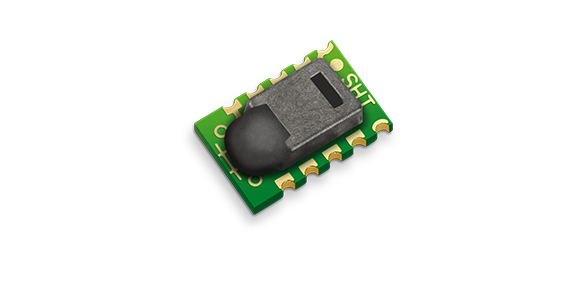
\includegraphics[width=5cm]{Imagenes/sht11_1.png} }}%
    \subfloat[\centering Cápsula permeable.]{{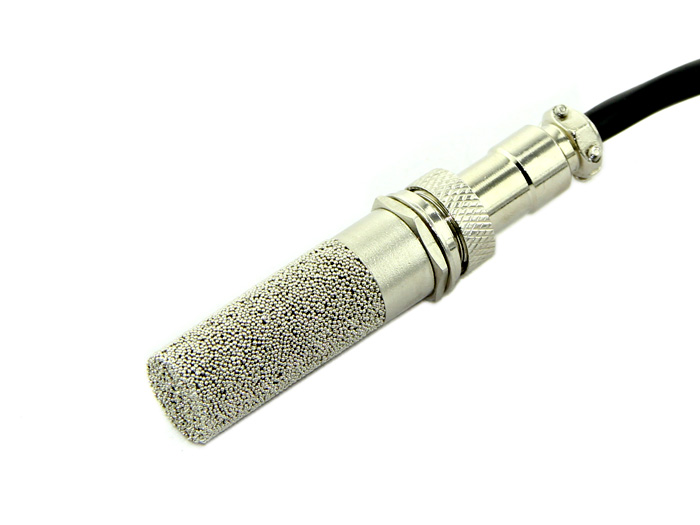
\includegraphics[width=5cm]{Imagenes/sht11.jpg} }}%
    \caption{Sensores resistivos implementados.}%
    \label{fig:sht11}%
\end{figure}

En las primeras experiencias realizadas procedimos a probar el sensor en tierra completamente disecada en un horno, donde arrojó una medición certera de 0\% de humedad. Luego la regamos hasta el punto de que quedó completamente irrigada, donde se midió un 99\% de humedad. Hasta este momento todo parecía funcionar perfectamente, pero nos encontramos con que los valores de humedad que arrojaba el sensor, seguían siendo altos incluso después de que la tierra se secara. Al inspeccionar con mas detalle, encontramos que dentro de la cápsula en la que se encuentra el mismo se había formado condensación por la elevada humedad del aire en su interior, la cual alteraba las mediciones realizadas, por lo que luego de mucha investigación optamos por modificar la cápsula misma, reemplazándola por una de mayor tamaño. Esto solucionó nuestros inconvenientes, ya que al haber un mayor volumen de aire no llegaba a formarse condensación sobre nuestro sensor, manteniendo lecturas adecuadas y preservando la durabilidad y robustez del sistema, motivo por el cual decidimos emplearlo para el desarrollo del proyecto.

\section{Diagrama de Bloque}

\centering
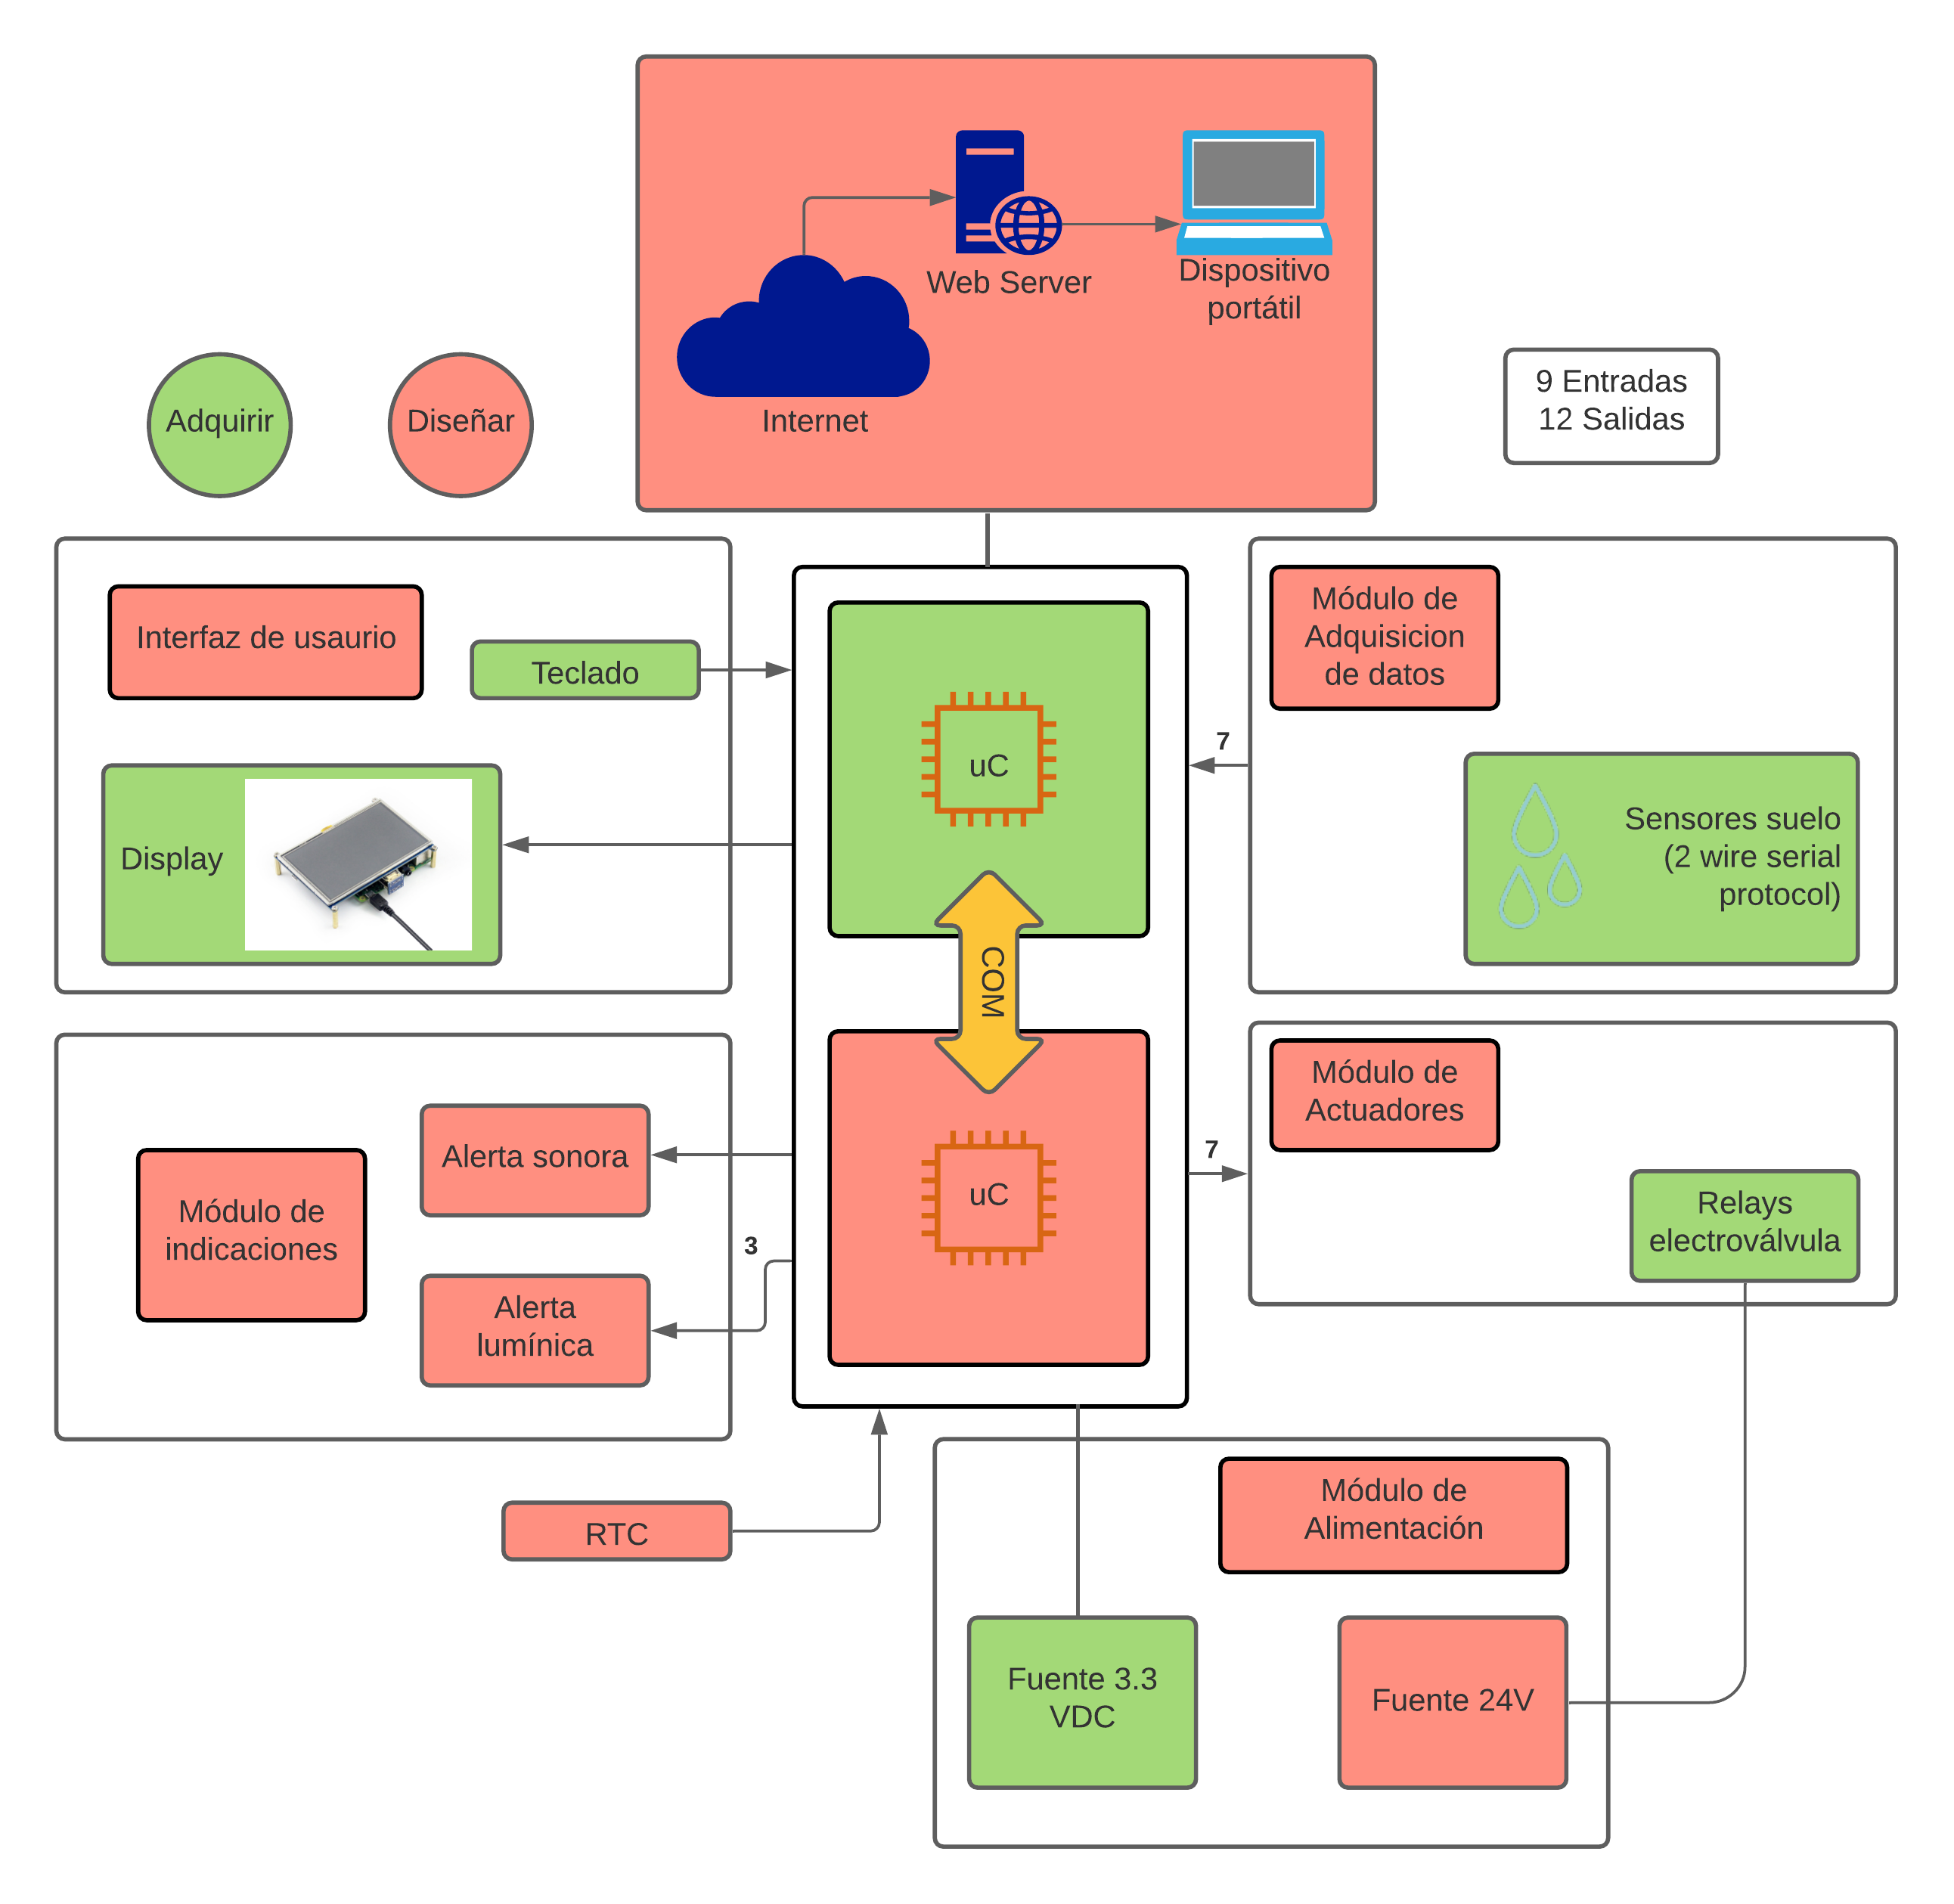
\includegraphics[width=\linewidth]{Imagenes/DIAGRAMA.png} \par
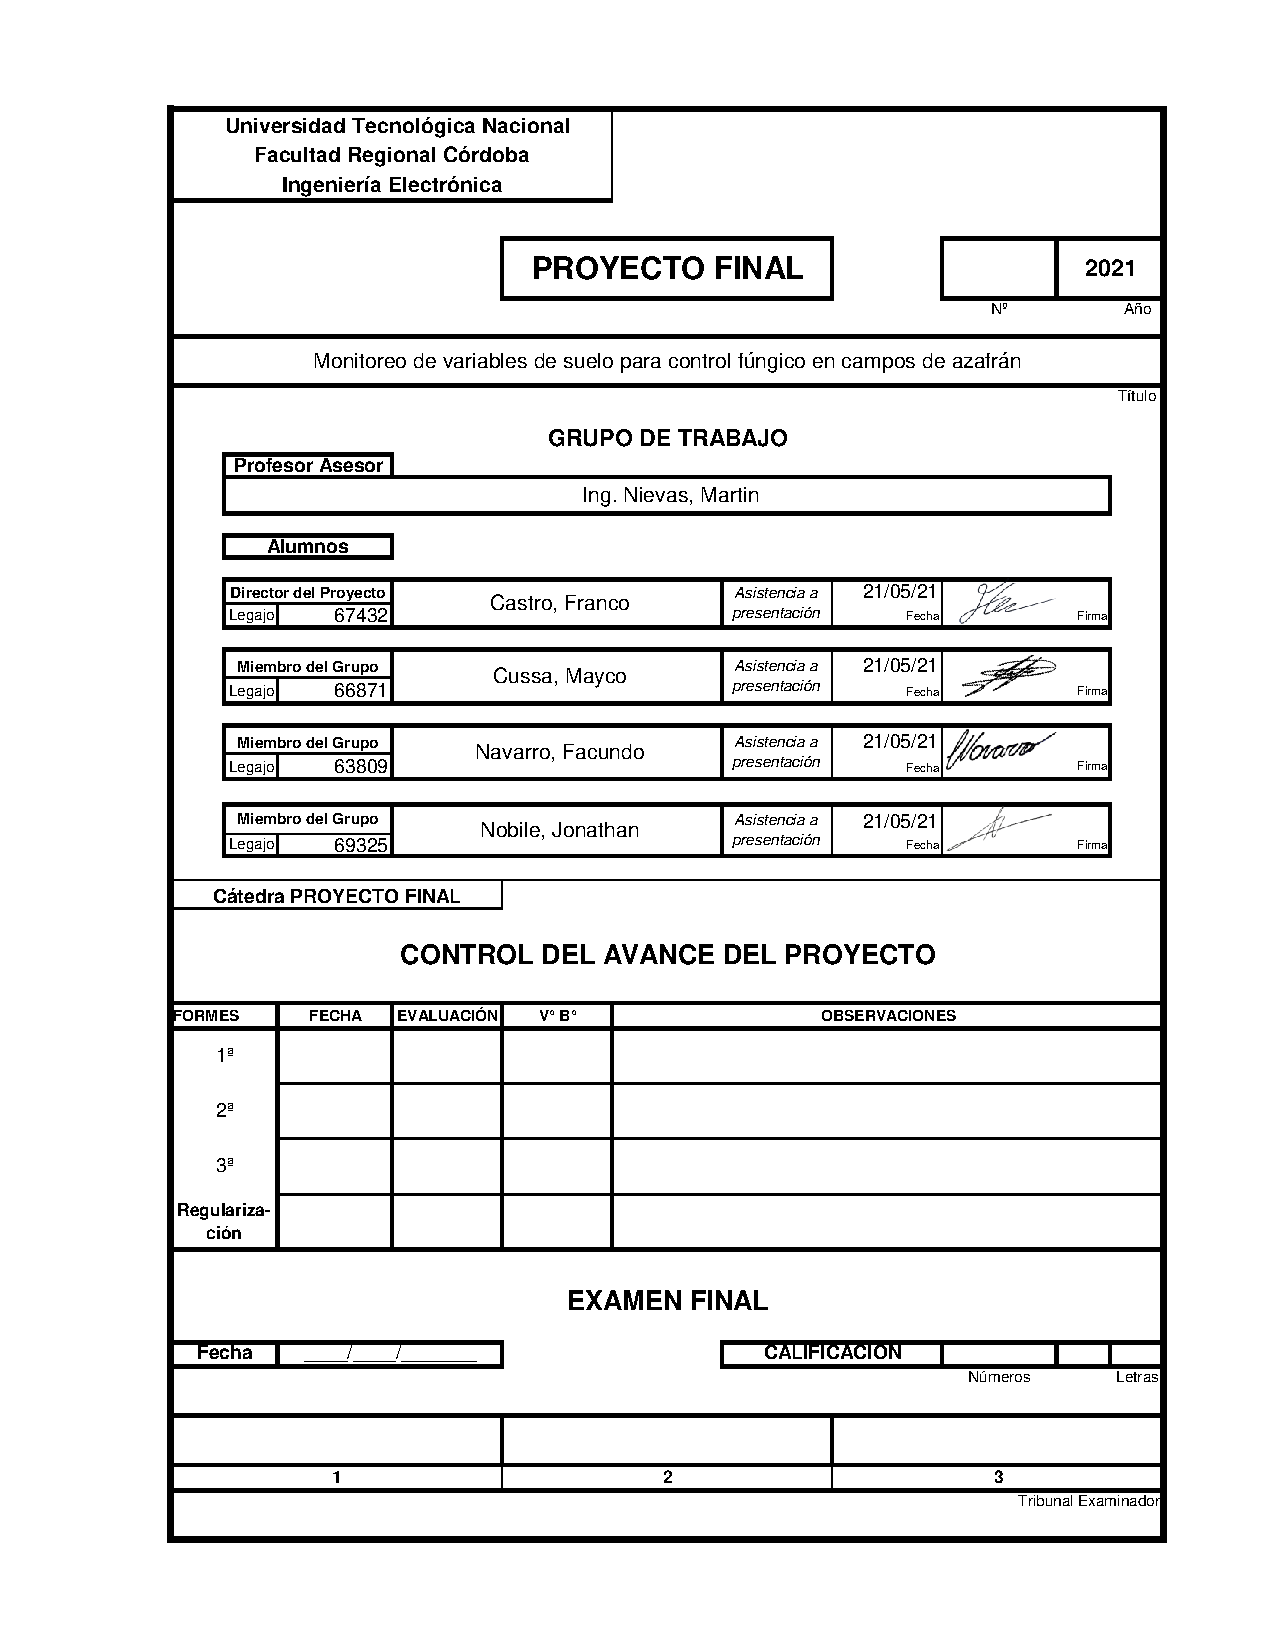
\includepdf[pages=-]{Caratula_Tesis_2021.pdf}
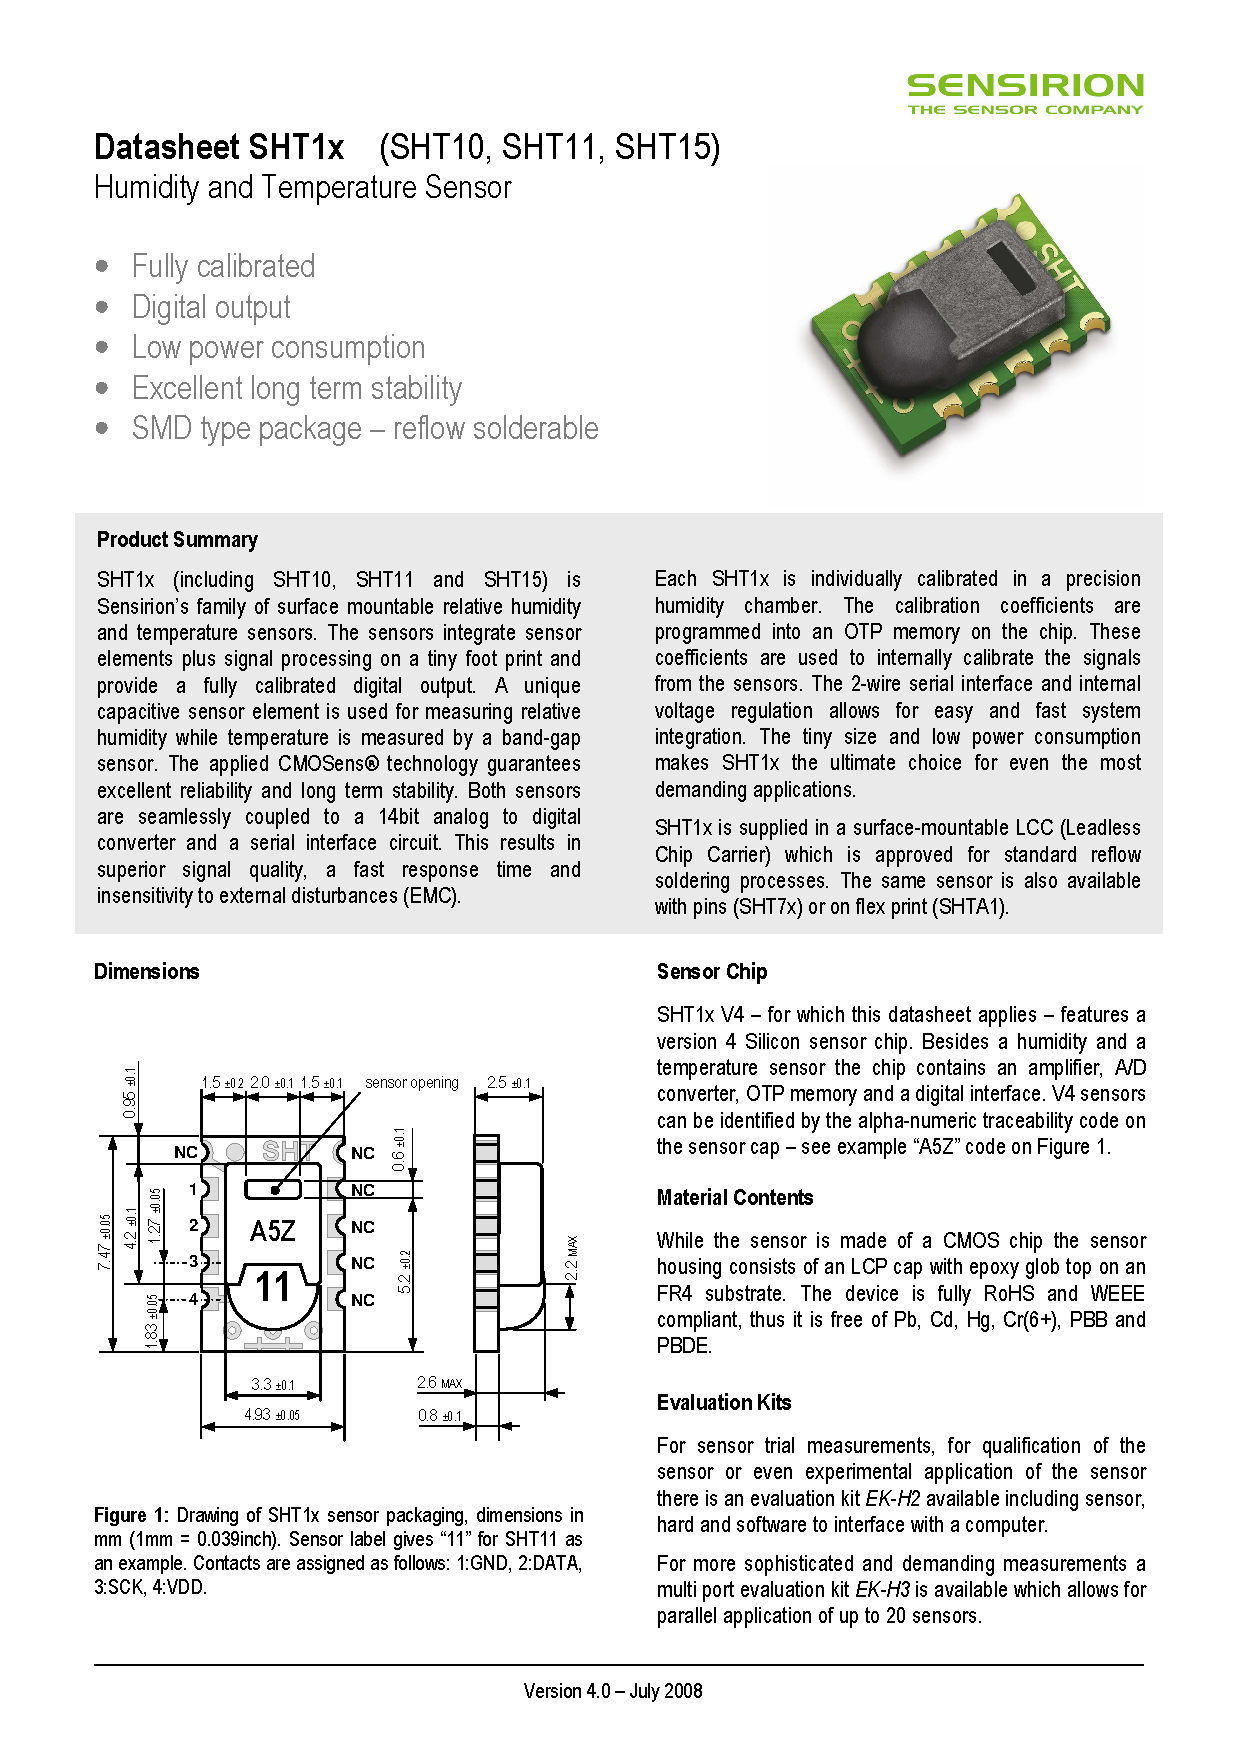
\includepdf[pages=1]{SHT1x_datasheet.pdf}
\includepdf[pages=2]{SHT1x_datasheet.pdf}
\end{document}